\chapter{Classification}

\begin{description}
    \item[(Supervised) classification] \marginnote{Classification} 
        Given a finite set of classes $C$ and a dataset $\matr{X}$ of $N$ individuals, 
        each associated to a class $y(\vec{x}) \in C$,
        we want to learn a model $\mathcal{M}$ able to 
        guess the value of $y(\bar{\vec{x}})$ for unseen individuals.

        Classification can be:
        \begin{descriptionlist}
            \item[Crisp] \marginnote{Crisp classification}
                Each individual has one and only one label.
            \item[Probabilistic] \marginnote{Probabilistic classification}
                Each individual is assigned to a label with a certain probability.
        \end{descriptionlist}

    \item[Classification model] \marginnote{Classification model}
        A classification model (classifier) makes a prediction by taking as input 
        a data element $\vec{x}$ and a decision function $y_\vec{\uptheta}$ parametrized on $\vec{\uptheta}$:
        \[ \mathcal{M}(\vec{x}, \vec{\uptheta}) = y_\vec{\uptheta}(\vec{x}) \]

    \item[Vapnik-Chervonenkis dimension] \marginnote{Vapnik-Chervonenkis dimension}
        A dataset with $N$ elements defines $2^N$ learning problems.
        A model $\mathcal{M}$ has Vapnik-Chervonenkis (VC) dimension $N$ if 
        it is able to solve all the possible learning problems with $N$ elements.

        \begin{example}
            A straight line has VC dimension 3.
        \end{example}

    \item[Data exploration] \marginnote{Data exploration}
        \begin{figure}[ht]
            \begin{subfigure}{.5\textwidth}
                \centering
                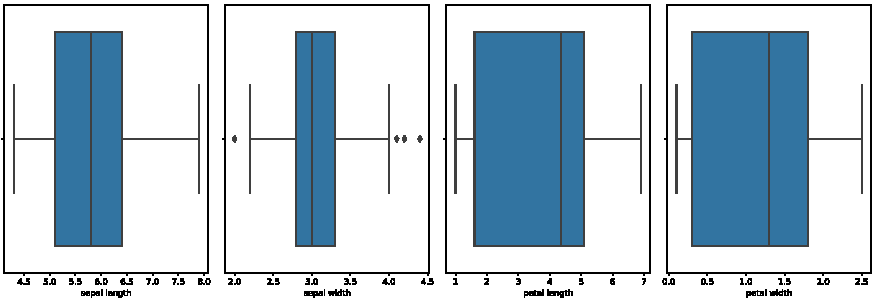
\includegraphics[width=\linewidth]{img/_iris_boxplot_general.pdf}
                \caption{Iris dataset general boxplot}
            \end{subfigure}%
            \begin{subfigure}{.5\textwidth}
                \centering
                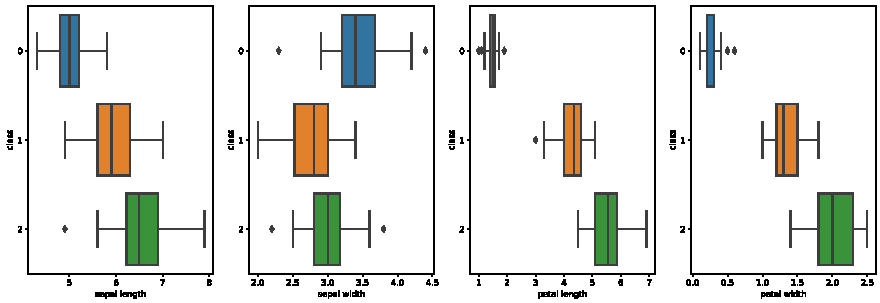
\includegraphics[width=\linewidth]{img/_iris_boxplot_inside.pdf}
                \caption{Iris dataset class boxplot}
            \end{subfigure}
            \begin{subfigure}{.5\textwidth}
                \centering
                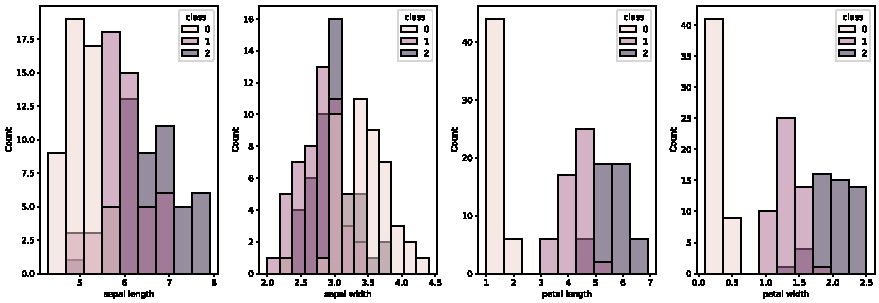
\includegraphics[width=\linewidth]{img/_iris_histogram.pdf}
                \caption{Iris dataset histograms}
            \end{subfigure}%
            \begin{subfigure}{.5\textwidth}
                \centering
                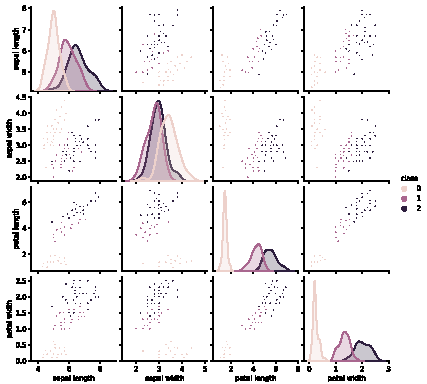
\includegraphics[width=\linewidth]{img/_iris_pairplot.pdf}
                \caption{Iris dataset pairplots}
            \end{subfigure}
        \end{figure}

    \item[Hyperparameters]
        Parameters of the model that have to be manually chosen.
\end{description}


\section{Evaluation}

\begin{description}
    \item[Dataset split]
        A supervised dataset can be randomly split into:
        \begin{descriptionlist}
            \item[Train set] \marginnote{Train set}
                Used to learn the model. Usually the largest split. Can be seen as an upper-bound of the model performance.
            \item[Test set] \marginnote{Test set}
                Used to evaluate the trained model. Can be seen as a lower-bound of the model performance.
            \item[Validation set] \marginnote{Validation set}
                Used to evaluate the model during training and/or for tuning parameters.
        \end{descriptionlist}
        It is assumed that the splits have similar characteristics.

    \item[Overfitting] \marginnote{Overfitting}
        Given a dataset $\matr{X}$, a model $\mathcal{M}$ is overfitting if
        there exists another model $\mathcal{M}'$ such that:
        \[ 
            \begin{split}
                \texttt{error}_\text{train}(\mathcal{M}) &< \texttt{error}_\text{train}(\mathcal{M}') \\
                \texttt{error}_\matr{X}(\mathcal{M}) &> \texttt{error}_\matr{X}(\mathcal{M}') \\
            \end{split}    
        \]

        Possible causes of overfitting are:
        \begin{itemize}
            \item Noisy data.
            \item Lack of representative instances.
        \end{itemize}
\end{description}


\subsection{Test set error}
\textbf{\underline{Disclaimer: I'm very unsure about this part}}\\
The error on the test set can be seen as a lower-bound error of the model.
If the test set error ratio is $x$, we can expect an error of $(x \pm  \text{confidence interval})$.

Predicting the elements of the test set can be seen as a binomial process (i.e. a series of $N$ Bernoulli processes).
We can therefore compute the empirical frequency of success as $f = (\text{correct predictions}/N)$.
We want to estimate the probability of success $p$.

We assume that the deviation between the empirical frequency and the true frequency is due to a 
normal noise around the true probability (i.e. the true probability $p$ is the mean).
Fixed a confidence level $\alpha$ (i.e. the probability of a wrong estimate),
we want that:
\[ \prob{ z_{\frac{\alpha}{2}} \leq \frac{f-p}{\sqrt{\frac{1}{N}p(1-p)}} \leq z_{(1-\frac{\alpha}{2})} } = 1 - \alpha \]
In other words, we want the middle term to have a high probability to 
be between the $\frac{\alpha}{2}$ and $(1-\frac{\alpha}{2})$ quantiles of the gaussian.
\begin{center}
    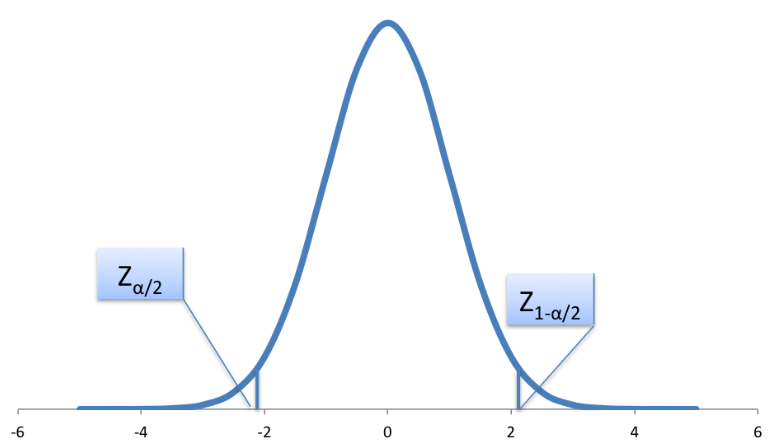
\includegraphics[width=0.4\textwidth]{img/normal_quantile_test_error.png}
\end{center}

We can estimate $p$ using the Wilson score interval\footnote{\url{https://en.wikipedia.org/wiki/Binomial_proportion_confidence_interval}}:
\[ p = \frac{1}{1+\frac{1}{N}z^2} \left( f + \frac{1}{2N}z^2 \pm z\sqrt{\frac{1}{N}f(1-f) + \frac{z^2}{4N^2}} \right) \]
where $z$ depends on the value of $\alpha$.
For a pessimistic estimate, $\pm$ becomes a $+$. Vice versa, for a optimistic estimate, $\pm$ becomes a $-$.

As $N$ is at the denominator, this means that for large values of $N$, the uncertainty becomes smaller.
\begin{center}
    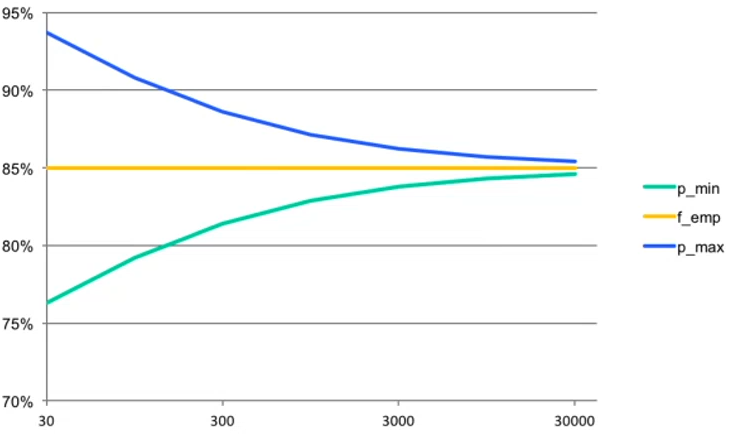
\includegraphics[width=0.45\textwidth]{img/confidence_interval.png}
\end{center}

\subsection{Dataset splits}

\begin{description}
    \item[Holdout] \marginnote{Holdout}
        The dataset is split into train, test and, if needed, validation.

    \item[Cross validation] \marginnote{Cross validation}
        The training data is partitioned into $k$ chunks.
        For $k$ iterations, one of the chunks if used to test and the others to train a new model.
        The overall error is obtained as the average of the errors of the $k$ iterations.

        At the end, the final model is still trained on the entire training data, 
        while cross validation results are used as an evaluation and comparison metric.
        Note that cross validation is done on the training set, so a final test set can still be used to
        evaluate the final model.

        \begin{figure}[h]
            \centering
            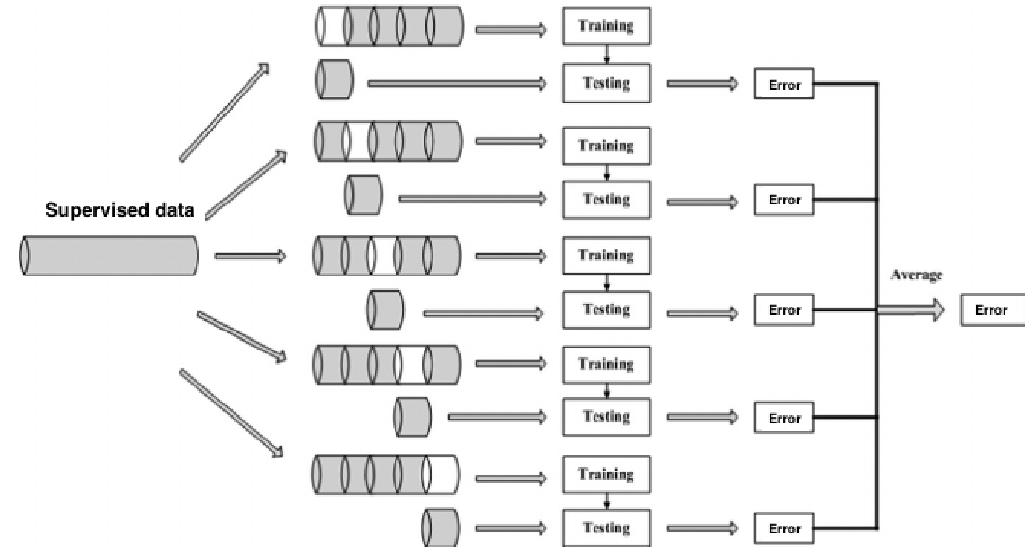
\includegraphics[width=0.6\textwidth]{img/cross_validation.png}
            \caption{Cross validation example}
        \end{figure}

    \item[Leave-one-out] \marginnote{Leave-one-out}
        Extreme case of cross validation with $k=N$, the size of the training set.
        In this case the whole dataset but one element is used for training and the remaining entry for testing.

    \item[Bootstrap] \marginnote{Bootstrap}
        Statistical sampling of the dataset with replacement (i.e. an entry can be selected multiple times).
        The selected entries form the training set while the elements that have never been selected are used for testing.
\end{description}


\subsection{Binary classification performance measures}

In binary classification, the two classes can be distinguished as the positive and negative labels.
The prediction of a classifier can be a:
\begin{center}
    True positive ($TP$) $\cdot$ False positive ($FP$) $\cdot$ True negative ($TN$) $\cdot$ False negative ($FN$)
\end{center}

\begin{center}
    \begin{tabular}{|c|c|c|c|}
        \cline{3-4}
        \multicolumn{2}{c|}{} & \multicolumn{2}{c|}{Predicted} \\
        \cline{3-4}
        \multicolumn{2}{c|}{} & Pos & Neg \\
        \hline
        \multirow{2}{*}{\rotatebox[origin=c]{90}{True}} & Pos & $TP$ & $FN$ \\
        \cline{2-4}
        & Neg & $FP$ & $TN$ \\
        \hline
    \end{tabular}
\end{center}

Given a test set of $N$ element, possible metrics are:
\begin{descriptionlist}
    \item[Accuracy] \marginnote{Accuracy}
        Number of correct predictions.
        \[ \text{accuracy} = \frac{TP + TN}{N} \]

    \item[Error rate] \marginnote{Error rate}
        Number of incorrect predictions.
        \[ \text{error rate} = 1 - \text{accuracy} \]

    \item[Precision] \marginnote{Precision}
        Number of true positives among what the model classified as positive
        (i.e. how many samples the model classified as positive are real positives).
        \[ \text{precision} = \frac{TP}{TP + FP} \]

    \item[Recall/Sensitivity] \marginnote{Recall}
        Number of true positives among the real positives
        (i.e. how many real positive the model predicted).
        \[ \text{recall} = \frac{TP}{TP + FN} \]

    \item[Specificity] \marginnote{Specificity}
        Number of true negatives among the real negatives
        (i.e. recall for negative labels).
        \[ \text{specificity} = \frac{TN}{TN + FP} \]

    \item[F1 score] \marginnote{F1 score}
        Harmonic mean of precision and recall
        (i.e. measure of balance between precision and recall).
        \[ \text{F1} = 2 \frac{\text{precision} \cdot \text{recall}}{\text{precision} + \text{recall}} \]
\end{descriptionlist}


\subsection{Multi-class classification performance measures}

\begin{descriptionlist}
    \item[Confusion matrix] \marginnote{Confusion matrix}
        Matrix to correlate the predictions of $n$ classes:
        \begin{center}
            \begin{tabular}{|c|c|c|c|c|c|}
                \cline{3-6}
                \multicolumn{2}{c|}{} & \multicolumn{4}{c|}{Predicted} \\
                \cline{3-6}
                \multicolumn{2}{c|}{} & a & b & c & Total \\
                \hline
                \multirow{4}{*}{\rotatebox[origin=c]{90}{True}} 
                & a & $TP_a$ & $FP_{a-b}$ & $FP_{a-c}$ & $T_a$ \\
                \cline{2-6}
                & b & $FP_{b-a}$ & $TP_b$ & $FP_{b-c}$ & $T_b$ \\
                \cline{2-6}
                & c & $FP_{c-a}$ & $FP_{c-b}$ & $TP_c$ & $T_c$ \\
                \cline{2-6}
                & Total & $P_a$ & $P_b$ & $P_c$ & $N$ \\
                \hline
            \end{tabular}
        \end{center}
        where:
        \begin{itemize}
            \item $a$, $b$ and $c$ are the classes.
            \item $T_x$ is the true number of labels of class $x$ in the dataset.
            \item $P_x$ is the predicted number of labels of class $x$ in the dataset.
            \item $TP_x$ is the number of times a class $x$ was correctly predicted (true predictions).
            \item $FP_{i-j}$ is the number of times a class $i$ was predicted as $j$ (false predictions).
        \end{itemize}

    \item[Accuracy] \marginnote{Accuracy}
        Accuracy is extended from the binary case as:
        \[ \text{accuracy} = \frac{\sum_i TP_i}{N} \]

    \item[Precision] \marginnote{Precision}
        Precision is defined w.r.t. a single class:
        \[ \text{precision}_i = \frac{TP_i}{P_i} \]

    \item[Recall] \marginnote{Recall}
        Recall is defined w.r.t. a single class:
        \[ \text{recall}_i = \frac{TP_i}{T_i} \]
\end{descriptionlist}

If a single value of precision or recall is needed, the mean can be used by computing
a macro (unweighted) average or a class-weighted average.

\begin{description}
    \item[$\kappa$-statistic] \marginnote{$\kappa$-statistic}
        Evaluates the concordance between two classifiers (in our case, the predictor and the ground truth).
        It is based on two probabilities:
        \begin{descriptionlist}
            \item[Probability of concordance] $\prob{c} = \frac{\sum_{i}^{\texttt{classes}} TP_i}{N}$ 
            \item[Probability of random concordance] $\prob{r} = \frac{\sum_{i}^{\texttt{classes}} T_i P_i}{N^2}$ 
        \end{descriptionlist}

        $\kappa$-statistic is given by:
        \[ \kappa = \frac{\prob{c} - \prob{r}}{1 - \prob{r}} \in [-1, 1] \]
        When $\kappa = 1$, there is perfect agreement ($\sum_{i}^{\texttt{classes}} TP_i = 1$), 
        when $\kappa = -1$, there is total disagreement ($\sum_{i}^{\texttt{classes}} TP_i = 0$) and
        when $\kappa = 0$, there is random agreement.
\end{description}


\subsection{Probabilistic classifier performance measures}

\begin{description}
    \item[Lift chart] \marginnote{Lift chart}
        Used in binary classification.
        Given the resulting probabilities of the positive class of a classifier, 
        sort them in decreasing order and plot a 2d-chart with
        increasing sample size on the x-axis and the number of positive samples on the y-axis.

        Then, plot a straight line to represent a baseline classifier that makes random choices.
        As the probabilities are sorted in decreasing order, it is expected a high concentration of
        positive labels on the right side.
        When the area between the two curves is large and the curve is above the random classifier, 
        the model can be considered a good classifier.

        \begin{figure}[h]
            \centering
            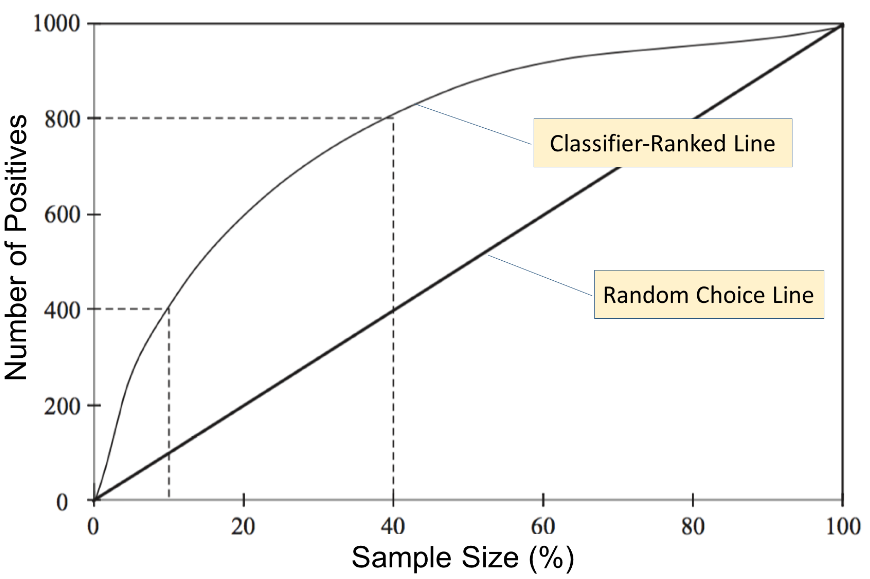
\includegraphics[width=0.5\textwidth]{img/lift_chart.png}
            \caption{Example of lift chart}
        \end{figure}

    \item[ROC curve] \marginnote{ROC curve}
        The ROC curve can be seen as a way to represent multiple confusion matrices of a classifier
        that uses different thresholds.
        The x-axis of a ROC curve represent the false positive rate while the y-axis represent the true positive rate.

        A straight line is used to represent a random classifier.
        A threshold can be considered good if it is high on the y-axis and low on the x-axis.
        
        \begin{figure}[h]
            \centering
            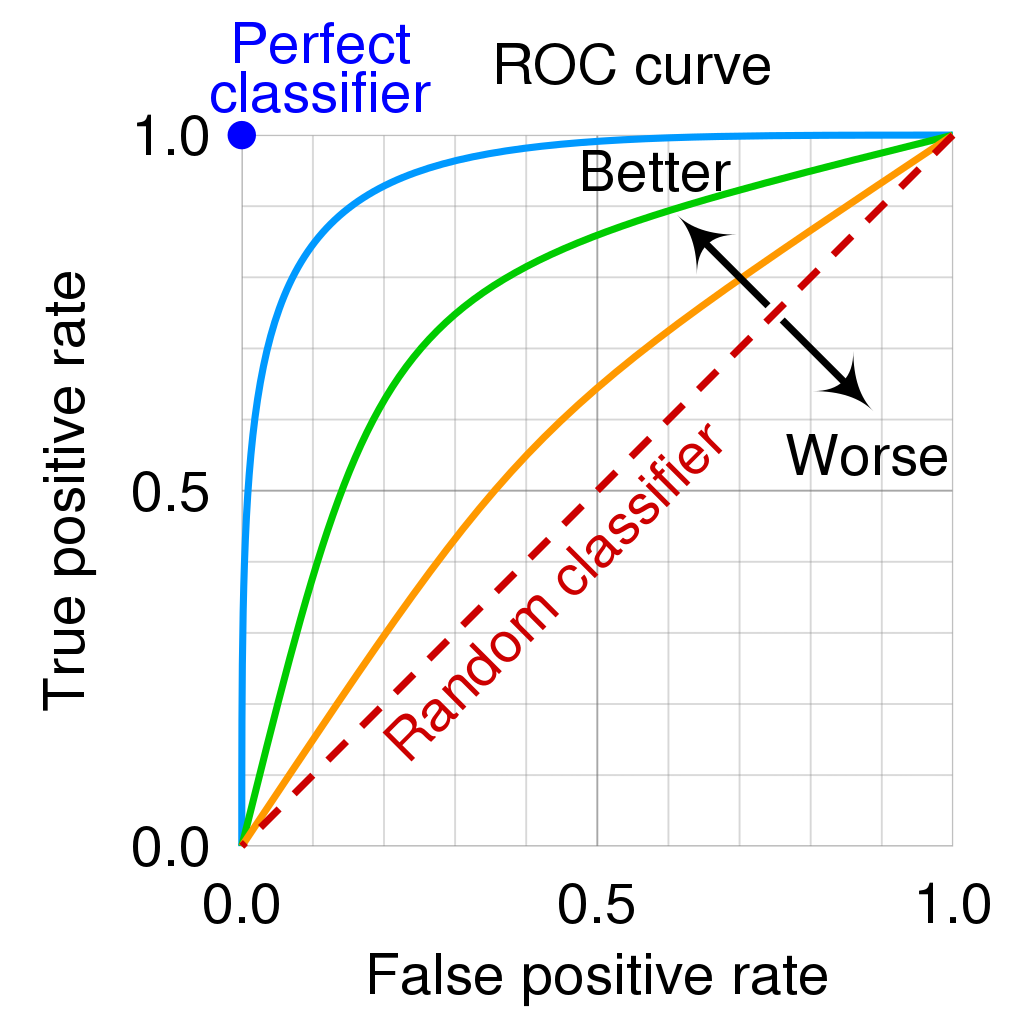
\includegraphics[width=0.35\textwidth]{img/roc_curve.png}
            \caption{Example of ROC curves}
        \end{figure}
\end{description}


\subsection{Data imbalance}
A classifier may not perform well when predicting a minority class of the training data.
Possible solutions are:
\begin{descriptionlist}
    \item[Undersampling] \marginnote{Undersampling}
        Randomly reduce the number of example of the majority classes.

    \item[Oversampling] \marginnote{Oversampling}
        Increase the examples of the minority classes.

        \begin{description}
            \item[Synthetic minority oversampling technique (SMOTE)] \marginnote{SMOTE}
                \begin{enumerate}
                    \item Randomly select an example $x$ belonging to the minority class.
                    \item Select a random neighbor $z_i$ among its $k$-nearest neighbors $z_1, \dots, z_k$.
                    \item Synthetize a new example by selecting a random point of the feature space between $x$ and $z_i$.
                \end{enumerate}
        \end{description}

    \item[Cost sensitive learning] \marginnote{Cost sensitive learning}
        Assign a cost to the errors. Higher weights are assigned to minority classes.
        This can be done by:
        \begin{itemize}
            \item Altering the proportions of the dataset by duplicating samples to reduce its misclassification.
            \item Weighting the classes (possible in some algorithms).
        \end{itemize}
\end{descriptionlist}



\section{Decision trees}

\subsection{Information theory} \label{sec:information_theory}

\begin{description}
    \item[Shannon theorem] \marginnote{Shannon theorem}
        Let $\matr{X} = \{ \vec{v}_1, \dots, \vec{v}_V \}$ be a data source where 
        each of the possible value has probability $p_i = \prob{\vec{v}_i}$.
        The best encoding allows to transmit $\matr{X}$ with 
        an average number of bits given by the \textbf{entropy} of $X$: \marginnote{Entropy}
        \[ H(\matr{X}) = - \sum_j p_j \log_2(p_j) \]
        $H(\matr{X})$ can be seen as a weighted sum of the surprise factor $-\log_2(p_j)$.
        If $p_j \sim 1$, then the surprise of observing $\vec{v}_j$ is low, vice versa,
        if $p_j \sim 0$, the surprise of observing $\vec{v}_j$ is high.
        
        Therefore, when $H(\matr{X})$ is high, $\matr{X}$ is close to an uniform distribution.
        When $H(\matr{X})$ is low, $\matr{X}$ is close to a constant.

        \begin{example}[Binary source] \phantom{}\\
            \begin{minipage}{.50\linewidth}
                The two values of a binary source $\matr{X}$ have respectively probability $p$ and $(1-p)$.
                When $p \sim 0$ or $p \sim 1$, $H(\matr{X}) \sim 0$.\\
                When $p \sim 0.5$, $H(\matr{X}) \sim \log_2(2)=1$
            \end{minipage}
            \begin{minipage}{.45\linewidth}
                \centering
                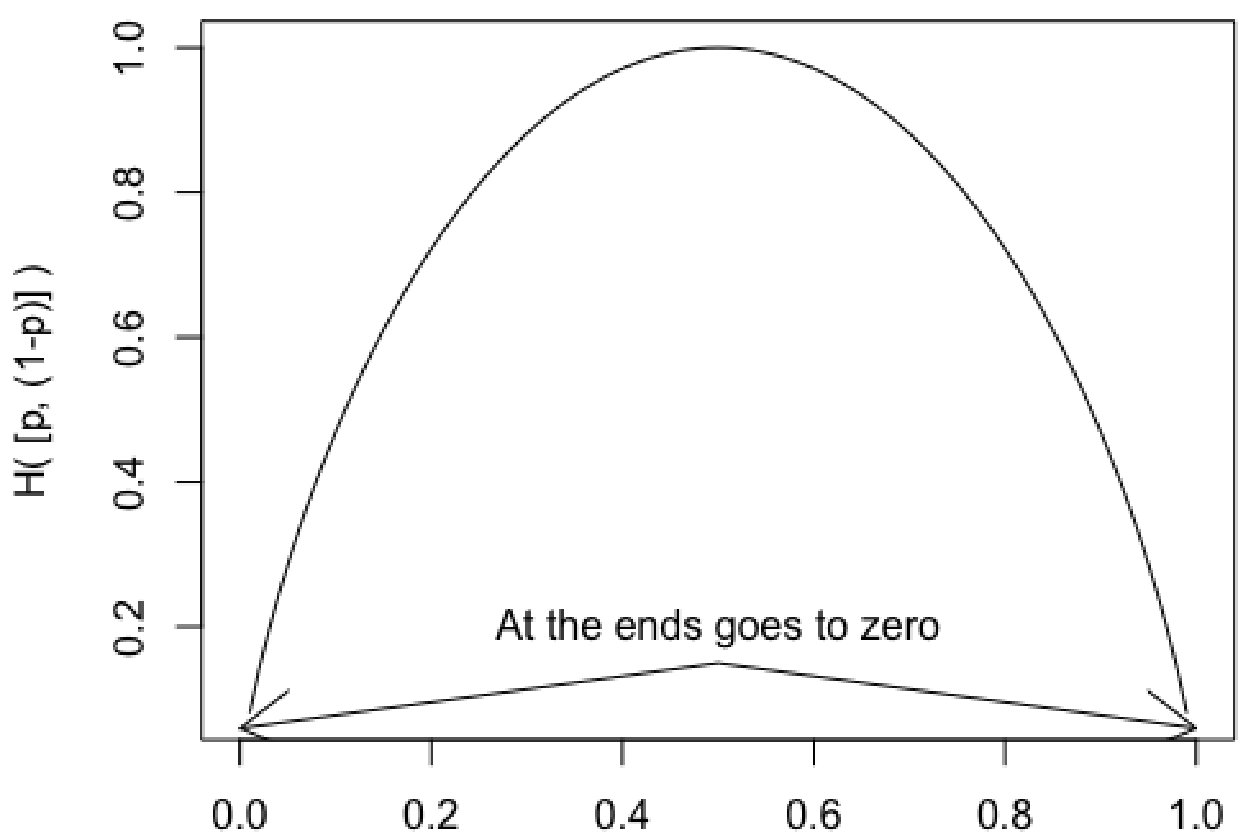
\includegraphics[width=\linewidth]{img/binary_entropy.png}
            \end{minipage}
        \end{example}

    \item[Entropy threshold split] \marginnote{Entropy threshold split}
        Given a dataset $\matr{D}$, 
        a real-valued attribute $d \in \matr{D}$,
        a threshold $t$ in the domain of $d$ and
        the class attribute $c$ of $\matr{D}$.
        The entropy of the class $c$ of the dataset $\matr{D}$ split with threshold $t$ on $d$ is a weighted sum:
        \[ H(c \,\vert\, d \,:\, t) = \prob{d < t}H(c \,\vert\, d < t) + \prob{d \geq t}H(c \,\vert\, d \geq t) \]

    \item[Information gain] \marginnote{Information gain}
        Information gain measures the reduction in entropy after applying a split.
        It is computed as:
        \[ IG(c \,\vert\, d \,:\, t) = H(c) - H(c \,\vert\, d \,:\, t) \]
        When $H(c \,\vert\, d \,:\, t)$ is low, $IG(c \,\vert\, d \,:\, t)$ is high 
        as splitting with threshold $t$ result in purer groups.
        Vice versa, when $H(c \,\vert\, d \,:\, t)$ is high, $IG(c \,\vert\, d \,:\, t)$ is low
        as splitting with threshold $t$ is not very useful.

        The information gain of a class $c$ split on a feature $d$ is given by:
        \[ IG(c \,\vert\, d) = \max_t IG(c \,\vert\, d \,:\, t) \]
\end{description}


\subsection{Tree construction}

\begin{description}
    \item[Decision tree (C4.5)] \marginnote{Decision tree}
        Tree-shaped classifier where leaves are class predictions and 
        inner nodes represent conditions that guide to a leaf.
        This type of classifier is non-linear (i.e. does not represent a linear separation).

        Each node of the tree contains:
        \begin{itemize}
            \item The applied splitting criteria (i.e. feature and threshold). 
                Leaves do not have this value.
            \item The purity (e.g. entropy) of the current split.
            \item Dataset coverage of the current split.
            \item Classes distribution.
        \end{itemize}

        \begin{figure}[h]
            \centering
            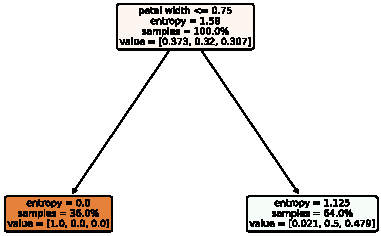
\includegraphics[width=0.5\textwidth]{img/_iris_decision_tree_example.pdf}
            \caption{Example of decision tree}
        \end{figure}

        Note: the weighted sum of the entropies of the children is always smaller than the entropy of the parent.

        Possible stopping conditions are:
        \begin{itemize}
            \item When most of the leaves are pure (i.e. nothing useful to split).
            \item When some leaves are impure but none of the possible splits have positive $IG$.
                Impure leaves are labeled with the majority class.
        \end{itemize}

    \item[Purity] \marginnote{Purity}
        Value to maximize when splitting a node of a decision tree.

        Nodes with uniformly distributed classes have a low purity.
        Nodes with a single class have the highest purity.

        Possible impurity measures are:
        \begin{descriptionlist}
            \item[Entropy/Information gain] See \Cref{sec:information_theory}. 

            \item[Gini index] \marginnote{Gini index}
                Let $\matr{X}$ be a dataset with classes $C$.
                The Gini index measures how often an element of $\matr{X}$ would be misclassified
                if the labels were randomly assigned based on the frequencies of the classes in $\matr{X}$.

                Given a class $i \in C$, $p_i$ is the probability (i.e. frequency) of classifying an element with $i$ and
                $(1 - p_i)$ is the probability of classifying it with a different label.
                The Gini index is given by:
                \[
                    \begin{split}
                        GINI(\matr{X}) = \sum_i^C p_i (1-p_i) &= \sum_i^C p_i - \sum_i^C p_i^2 \\
                            &= 1 - \sum_i^C p_i^2
                    \end{split}  
                \]
                When $\matr{X}$ is uniformly distributed, $GINI(\matr{X}) \sim (1-\frac{1}{\vert C \vert})$.
                When $\matr{X}$ is constant, $GINI(\matr{X}) \sim 0$.

                Given a node $x$ split in $n$ children $x_1, \dots, x_n$,
                the Gini gain of the split is given by:
                \[ GINI_\text{gain} = GINI(x) - \sum_{i=1}^n \frac{\vert x_i \vert}{\vert x \vert} GINI(x_i) \]
 
            \item[Misclassification error] \marginnote{Misclassification error}
                Skipped.
        \end{descriptionlist}

        \begin{figure}[h]
            \centering
            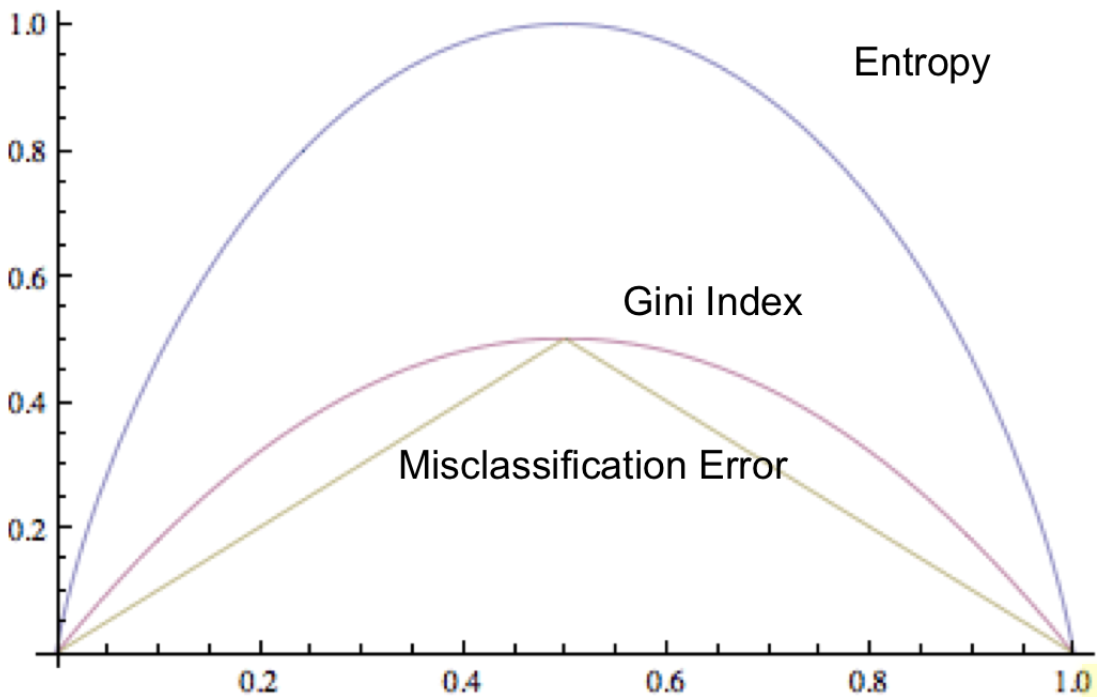
\includegraphics[width=0.35\textwidth]{img/impurity_comparison.png}
            \caption{Comparison of impurity measures}
        \end{figure}

        Compared to Gini index, entropy is more robust to noise.

        Misclassification error has a bias toward the major class.
\end{description}

\begin{algorithm}[H]
\caption{Decision tree construction using information gain as impurity measure}
\begin{lstlisting}
    def buildTree(split):
        node = Node()
        if len(split.classes) == 1: # Pure split
            node.label = split.classes[0]
            node.isLeaf = True
        else:
            ig, attribute, threshold = getMaxInformationGain(split)
            if ig < 0:
                node.label = split.majorityClass()
                node.isLeaf = True
            else:
                node.left = buildTree(split[attribute < threshold])
                node.right = buildTree(split[attribute >= threshold])
        return node
\end{lstlisting}
\end{algorithm}

\begin{description}
    \item[Pruning] \marginnote{Pruning}
        Remove branches to reduce overfitting.
        Different pruning techniques can be employed:
        \begin{descriptionlist}
            \item[Maximum depth] 
                Maximum depth allowed for the tree.

            \item[Minimum samples for split] 
                Minimum number of samples a node is required to have to apply a split.

            \item[Minimum samples for a leaf] 
                Minimum number of samples a node is required to have to become a leaf.

            \item[Minimum impurity decrease] 
                Minimum decrease in impurity for a split to be made.

            \item[Statistical pruning] 
                Prune the children of a node if the weighted sum of the maximum errors of the children is greater than 
                the maximum error of the node if it was a leaf.
        \end{descriptionlist}
\end{description}


\subsection{Complexity}
Given a dataset $\matr{X}$ of $N$ instances and $D$ attributes,
each level of the tree requires to evaluate all the dataset and
each node requires to process all the attributes.
Assuming an average height of $O(\log N)$, 
the overall complexity for induction (parameters search) is $O(DN \log N)$.

Moreover, The other operations of a binary tree have complexity:
\begin{itemize}
    \item Threshold search and binary split: $O(N \log N)$ (scan the dataset for the threshold).
    \item Pruning: $O(N \log N)$ (requires to scan the dataset).
\end{itemize}

For inference, to classify a new instance it is sufficient to traverse the tree from the root to a leaf.
This has complexity $O(h)$, with $h$ the height of the tree.


\subsection{Characteristics}
\begin{itemize}
    \item Decision trees are non-parametric in the sense that they do not require any assumption on the distribution of the data.
    \item Finding the best tree is an NP-complete problem.
    \item Decision trees are robust to noise if appropriate overfitting methods are applied.
    \item Decision trees are robust to redundant attributes (correlated attributes are very unlikely to be chosen for multiple splits).
    \item In practice, the impurity measure has a low impact on the final result, while the pruning strategy is more relevant.
\end{itemize}



\section{Naive Bayes}

\begin{description}
    \item[Bayes' theorem]
        Given a class $c$ and the evidence $\vec{e}$, we have that:
        \[ \prob{c \mid \vec{e}} = \frac{\prob{\vec{e} \mid c} \prob{c}}{\prob{\vec{e}}} \]

    \item[Naive Bayes classifier] \marginnote{Naive Bayes classifier}
        Classifier that uses the Bayes' theorem assuming that the attributes are independent given the class.
        Given a class $c$ and the evidence $\vec{e} = \langle e_1, e_2, \dots, e_n \rangle$, the probability that 
        the observation $\vec{e}$ is of class $c$ is given by:
        \[
            \prob{c \mid \vec{e}} = \frac{\prod_{i=1}^{n}\prob{e_i \mid c} \cdot \prob{c}}{\prob{\vec{e}}}  
        \]
        As the denominator is the same for all classes, it can be omitted.
\end{description}


\subsection{Training and inference}
\begin{description}
    \item[Training] \marginnote{Training} 
        Given the classes $C$ and the features $E$,
        to train the classifier the following priors need to be estimated:
        \begin{itemize}
            \item $\forall c \in C:\, \prob{c}$
            \item $\forall e_{ij} \in E, \forall c \in C:\, \prob{e_{ij} \mid c}$,
                where $e_{ij}$ is the $j$-th value of the domain of the $i$-th feature $E_i$.
        \end{itemize}

    \item[Inference] \marginnote{Inference} 
        Given a new observation $\vec{x}_\text{new} = \langle x_1, x_2, \dots, x_n \rangle$,
        its class is determined by computing the likelihood:
        \[
            c_\text{new} = \arg\max_{c \in C} \prob{c} \prod_{i=1}^{n}\prob{x_i \mid c}
        \]
\end{description}


\subsection{Problems}
\begin{description}
    \item[Smooting] 
        If the value $e_{ij}$ of the domain of a feature $E_i$ never appears in the dataset, 
        its probability $\prob{e_{ij} \mid c}$ will be 0 for all classes.
        This nullifies all the probabilities that uses this feature when 
        computing the products chain during inference.
        Smoothing methods can be used to avoid this problem.

        \begin{description}
            \item[Laplace smoothing] \marginnote{Laplace smoothing}
                Given:
                \begin{descriptionlist}
                    \item[$\alpha$] The smoothing factor.
                    \item[\normalfont$\text{af}_{e_{ij}, c}$] The absolute frequency of the value $e_{ij}$ of the feature $E_i$ over the class $c$.
                    \item[$\vert \mathbb{D}_{E_i} \vert$] The number of distinct values in the domain of $E_i$.
                    \item[\normalfont$\text{af}_{c}$] The absolute frequency of the class $c$.
                \end{descriptionlist}
                the smoothed frequency is computed as:
                \[
                    \prob{e_{ij} \mid c} = \frac{\text{af}_{e_{ij}, c} + \alpha}{\text{af}_{c} + \alpha \vert \mathbb{D}_{E_i} \vert}    
                \]

                A common value of $\alpha$ is 1.
                When $\alpha = 0$, there is no smoothing.
                For higher values of $\alpha$, the smoothed feature gain more importance when computing the priors.
        \end{description}

    \item[Missing values] \marginnote{Missing values}
        Naive Bayes is robust to missing values.

        During training, the record is ignored in the frequency count of the missing feature.

        During inference, the missing feature can be simply excluded in the computation of the likelihood
        as this equally affects all classes.

    \item[Numeric values] \marginnote{Gaussian assumption}
        For continuous numeric values, the frequency count method cannot be used.
        Therefore, an additional assumption is made: numeric values follow a Gaussian distribution.

        During training, the mean $\mu_{i,c}$ and variance $\sigma_{i,c}$ for a numeric feature $E_i$ is computed with respect to a class $c$.
        Its probability is then obtained as:
        \[ \prob{E_i = x \mid c} = \mathcal{N}(\mu_{i,c}, \sigma_{i,c})(x) \]

\end{description}



\section{Perceptron}

\begin{description}
    \item[Perceptron] \marginnote{Perceptron}
        A single artificial neuron that takes $n$ inputs $x_1, \dots, x_n$ and a bias $b$,
        and computes a linear combination of them with weights $w_1, \dots, w_n, w_b$.
        \begin{figure}[h]
            \centering
            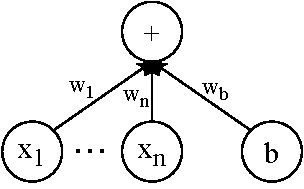
\includegraphics[width=0.25\textwidth]{img/_perceptron.pdf}
            \caption{Example of perceptron}
        \end{figure}

        The learnt weights $w_b, w_1, \dots, w_n$ define a hyperplane for binary classification such that:
        \[
            w_1 x_1 + \text{\dots} + w_n x_n + w_b b = \begin{cases}
                \texttt{positive} & \text{if $> 0$} \\
                \texttt{negative} & \text{if $< 0$} \\
            \end{cases}
        \]
        It can be shown that there are either none or infinite hyperplanes with this property.
\end{description}


\subsection{Training}
\begin{algorithm}
\caption{Perceptron training}
\begin{lstlisting}[mathescape=true]
    def trainPerceptron(dataset):
        perceptron = Perceptron(weights=[0 $\dots$ 0])
        
        while accuracy(perceptron, dataset) != 1.0:
            for x, y in dataset:
                if perceptron.predict(x) != y:
                    if y is positive_class:
                        perceptron.weights += x
                    else:
                        perceptron.weights -= x
\end{lstlisting}
\end{algorithm}

Note that the algorithm converges only if the dataset is linearly separable.
In practice, a maximum number of iterations is set.



\section{Support vector machine}

\begin{description}
    \item[Convex hull]
        The convex hull of a set of points is the tightest enclosing convex polygon that contains those points.

        Note: the convex hulls of a linearly separable dataset do not intersect.

    \item[Maximum margin hyperplane] \marginnote{Maximum margin hyperplane}
        Hyperplane with the maximum margin between two convex hulls.

        In general, a subset of points (support vectors) \marginnote{Support vectors} 
        in the training set is sufficient to define the hulls.

        \begin{figure}[h]
            \centering
            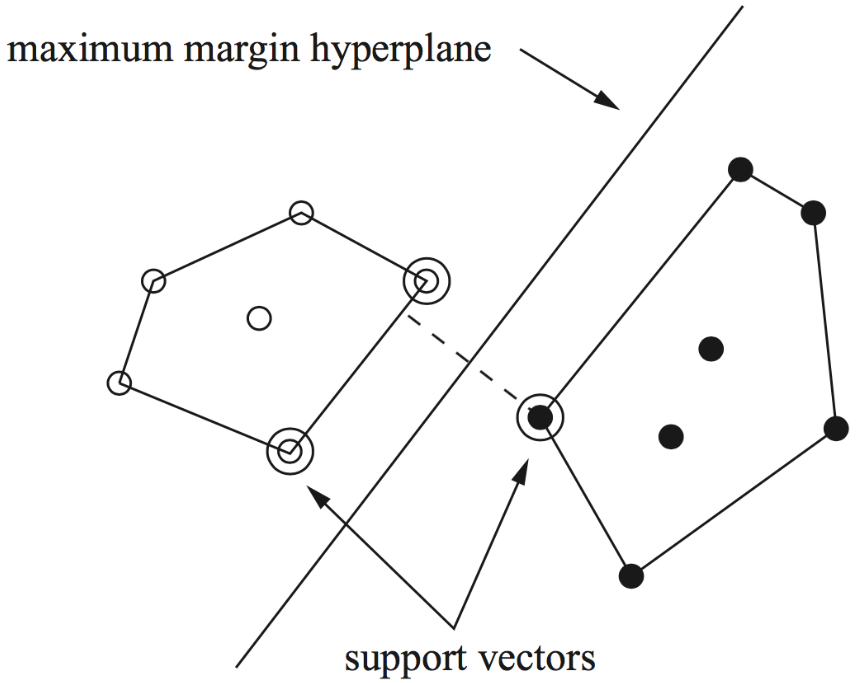
\includegraphics[width=0.4\textwidth]{img/svm.png}
            \caption{Maximum margin hyperplane of linearly separable data}
        \end{figure}

    \item[Support vector machine] \marginnote{Support vector machine}
        SVM\footnote{\scriptsize\url{https://www.cs.princeton.edu/courses/archive/spring16/cos495/slides/AndrewNg_SVM_note.pdf}} 
        finds the maximum margin hyperplane and the support vectors as a constrained quadratic optimization problem.
        Given a dataset of $D$ elements and $n$ features, the problem is defined as:
        \[ \max_{w_0, w_1, \dots, w_n} M \]
        \[ 
            \begin{split}
                \text{subject to }  & \sum_{i=1}^{n} w_i^2 = 1 \\
                                    & c_i(w_0 + w_1 x_{i1} + \dots + w_n x_{in}) \geq M \,\, \forall i = 1, \dots, D
            \end{split}    
        \]
        where $M$ is the margin, $w_i$ are the weights of the hyperplane and $c_i = \{-1, 1 \}$ is the class.
        The second constraint imposes the hyperplane to have a large margine. 
        For positive labels ($c_i=1$), this is true when the hyperplane is positive.
        For negative labels ($c_i=-1$), this is true when the hyperplane is negative.

        \begin{description}
            \item[Soft margin] \marginnote{Soft margin}
                As real-world data is not always linearly separable, 
                soft margin relaxes the margin constraint by adding a penalty $C$.
                The margin constraint becomes:
                \[ c_i(w_0 + w_1 x_{i1} + \dots + w_n x_{in}) \geq M - \xi_i \,\, \forall i = 1, \dots, D \]
                \[ \text{where } \xi_i \geq 0 \text{ and } \sum_{i=0}^{D} \xi_i = C \]
        \end{description}
\end{description}


\subsection{Kernel trick}\marginnote{Kernel trick}
For non-linearly separable data, the boundary can be found using a non-linear mapping 
to map the data into a new space (feature space) where a linear separation is possible.
Then, the data and the boundary is mapped back into the original space.

\begin{figure}[h]
    \begin{subfigure}{0.49\textwidth}
        \centering
        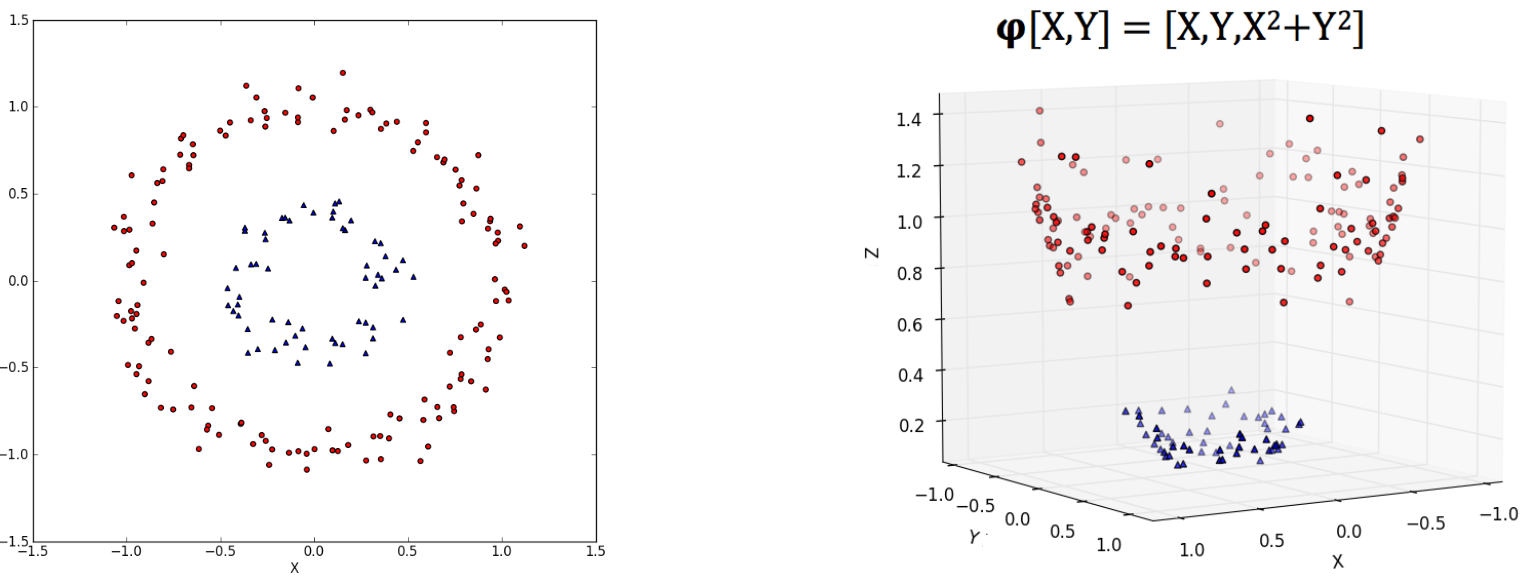
\includegraphics[width=\linewidth]{img/svm_kernel_example1.png}
    \end{subfigure}
    \begin{subfigure}{0.49\textwidth}
        \centering
        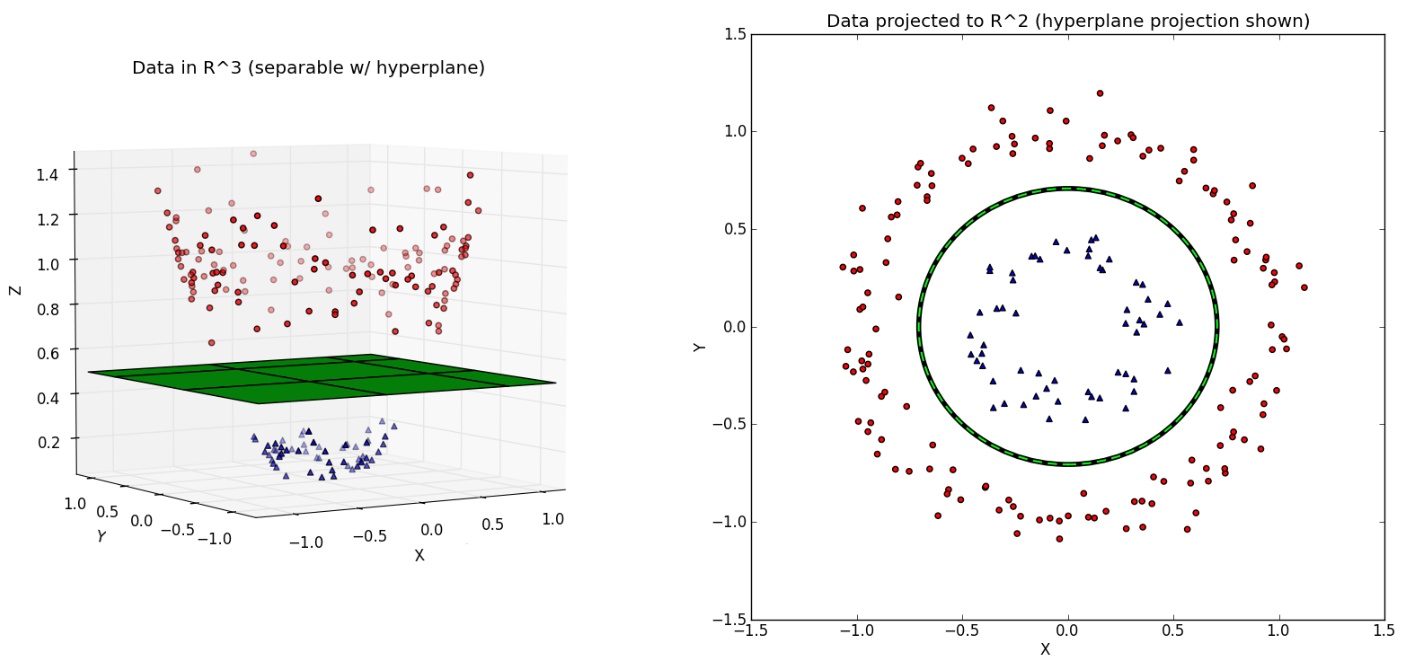
\includegraphics[width=\linewidth]{img/svm_kernel_example2.png}
    \end{subfigure}
    \caption{Example of mapping from $\mathbb{R}^2$ to $\mathbb{R}^3$}
\end{figure}

The kernel trick allows to avoid to explicitly map the dataset into the new space by using kernel functions.
Known kernel functions are:
\begin{descriptionlist}
    \item[Linear] $K(x, y) = \langle x, y \rangle$.
    \item[Polynomial] $K(x, y) = (\gamma \langle x, y \rangle + r)^d$, where $\gamma$, $r$ and $d$ are parameters.
    \item[Radial based function] $K(x, y) = \exp(-\gamma \Vert x - y \Vert^2)$, where $\gamma$ is a parameter.
    \item[Sigmoid] $K(x, y) = \tanh(\langle x, y \rangle + r)$, where $r$ is a parameter.
\end{descriptionlist}


\subsection{Complexity}
Given a dataset with $D$ entries of $n$ features, the complexity of SVM scales from $O(nD^2)$ to $O(nD^3)$
depending on the effectiveness of data caching.


\subsection{Characteristics}
\begin{itemize}
    \item Training an SVM model is generally slower.
    \item SVM is not affected by local minimums.
    \item SVM do not suffer the curse of dimensionality.
    \item SVM does not directly provide probability estimates. 
        If needed, these can be computed using a computationally expensive method.
\end{itemize}



\section{Neural networks}

\begin{description}
    \item[Multilayer perceptron] \marginnote{Multilayer perceptron}
        Hierarchical structure of perceptrons, each with an activation function.

    \item[Activation function] \marginnote{Activation function}
        Activation functions are useful to add non-linearity.

        In a linear system, if there is noise in the input, it is transferred to the output 
        (i.e. linearity implies that $f(x + \text{noise}) = f(x) + f(\text{noise})$).
        On the other hand, a non-linear system is generally more robust 
        (i.e. non-linearity generally implies that $f(x + \text{noise}) \neq f(x) + f(\text{noise})$)

    \item[Feedforward neural network] \marginnote{Feedforward neural network}
        Network with the following flow:
        \[ \text{Input layer} \rightarrow \text{Hidden layer} \rightarrow \text{Output layer} \]
        Neurons at each layer are connected to all neurons of the next layer.
\end{description}


\subsection{Training}
Inputs are fed to the network and backpropagation is used to update the weights.

\begin{description}
    \item[Learning rate] \marginnote{Learning rate}
        Size of the step for gradient descent.

    \item[Epoch] \marginnote{Epoch} 
        A round of training where the entire dataset has been processed.

    \item[Stopping criteria] \marginnote{Stopping criteria}
        Possible conditions to stop the training are:
        \begin{itemize}
            \item Small weights update.
            \item The classification error goes below a predefined target.
            \item Timeout or maximum number of epochs.
        \end{itemize}

    \item[Regularization] \marginnote{Regularization}
        Smoothing of the loss function.
\end{description}



\section{K-nearest neighbors}

\begin{description}
    \item[K-nearest neighbors] \marginnote{K-nearest neighbors}
        Given a similarity metric and a training set,
        to predict a new observation, the $k$ most similar entries in the training set are selected
        and the class of the new data is determined as the most frequent class among the $k$ entries.
\end{description}



\section{Binary to multi-class classification}

\begin{description}
    \item[One-vs-one strategy (OVO)] \marginnote{One-vs-one strategy (OVO)}
        Train a classifier for all the possible pairs of classes (this will result in $\frac{C \cdot (C-1)}{2}$ pairs).
        The class assigned to a new observation is determined through a majority vote.

    \item[One-vs-rest strategy (OVR)] \marginnote{One-vs-rest strategy (OVR)}
        Train $C$ classifiers where each is specialized to classify a specific class as positive and the others as negative.
        The class assigned to a new observation is determined by the confidence score of each classifier.
\end{description}



\section{Ensemble methods}
\marginnote{Ensemble methods}
Train a set of base classifiers and make predictions by majority vote.
If all the classifiers have the same but independent error rate, 
the overall error of the ensemble model is lower (derived from a binomial distribution).

\begin{figure}[h]
    \centering
    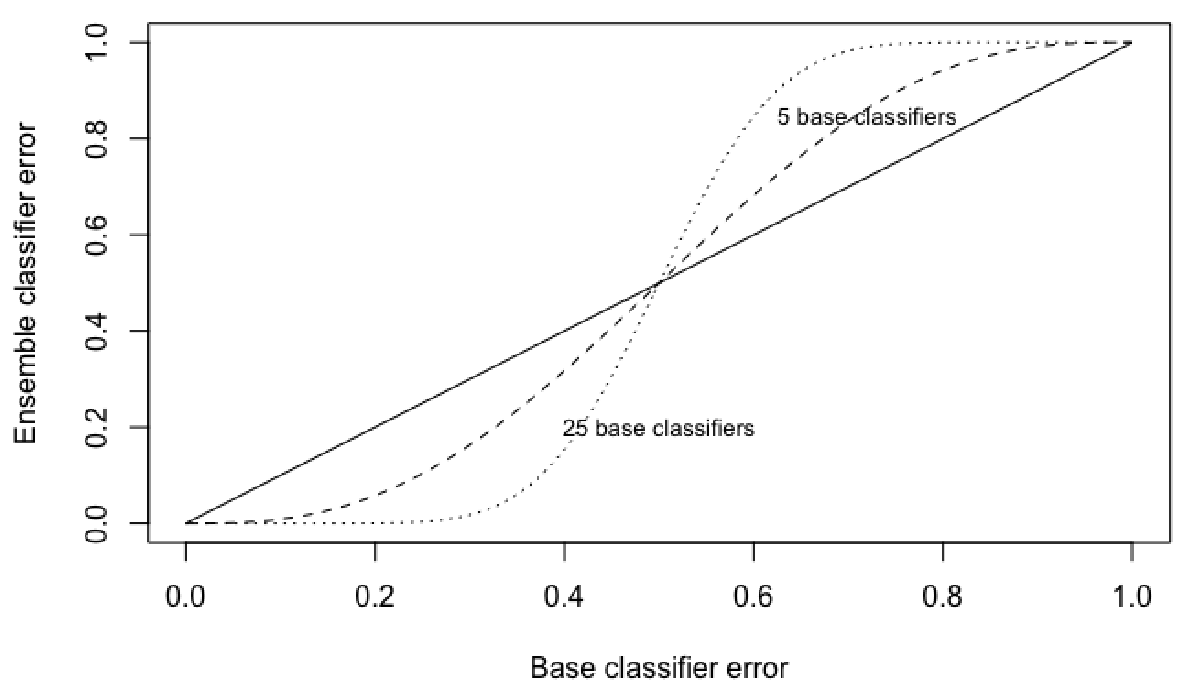
\includegraphics[width=0.6\textwidth]{img/ensemble_error.png}
    \caption{Relationship between the error of base classifiers and ensemble models}
\end{figure}

Different strategies to train an ensemble classifier can be used:
\begin{descriptionlist}
    \item[Dataset manipulation] Resampling the dataset for each base classifier:
        \begin{description}
            \item[Bagging] 
                Sample with replacement with a uniform distribution.
            \item[Boosting] 
                Iteratively change the distribution of the training data 
                prioritizing examples difficult to classify.
                \begin{description}
                    \item[Adaboost] \marginnote{Adaboost}
                        Iteratively train base classifiers on a dataset where samples 
                        misclassified at the previous iteration have a higher weight.
                \end{description}
        \end{description}
    
    \item[Feature manipulation]
        Train a base classifier using only a subset of the features.

    \item[Class labels manipulation]
        Train a base classifier to classify a partition of the class labels.
        For instance, class labels can be partitioned into two groups $A_1$ and $A_2$, and
        the base classifier is trained to assign as label one of the two groups.
        During inference, when a group is predicted, all labels within that group receive a vote.
\end{descriptionlist}


\subsection{Random forests}
\marginnote{Random forests}

Different decision trees trained on a different random sampling of the training set and different subset of features.
A prediction is made by averaging the output of each tree.

\begin{description}
    \item[Bias] \marginnote{Bias}
        Simplicity of the target function of a model.
    \item[Variance] \marginnote{Variance}
        Amount of change of the target function when using different training data (i.e. how much the model overfits).
\end{description}

Random forests aim to reduce the high variance of decision trees.